%% SoftwareX original software article
%% pyfieldml: a modern Python implementation of FieldML 0.5 for
%% computational biomechanics
%%
%% Compile with:
%%   pdflatex pyfieldml-softwarex
%%   bibtex   pyfieldml-softwarex
%%   pdflatex pyfieldml-softwarex
%%   pdflatex pyfieldml-softwarex
%%
%% or: make

\documentclass[preprint,12pt,a4paper]{elsarticle}

\usepackage{amssymb}
\usepackage[hyphens]{url}
\usepackage{hyperref}
\usepackage{graphicx}
\usepackage{listings}
\usepackage{xcolor}
\setlength{\parindent}{0pt}
\setlength{\parskip}{4pt}
\sloppy

\definecolor{codebg}{rgb}{0.97,0.97,0.97}
\definecolor{codekw}{rgb}{0.15,0.35,0.65}
\definecolor{codestr}{rgb}{0.20,0.55,0.20}
\definecolor{codecom}{rgb}{0.45,0.45,0.45}
\lstdefinestyle{pystyle}{
  language=Python,
  basicstyle=\ttfamily\footnotesize,
  backgroundcolor=\color{codebg},
  keywordstyle=\color{codekw}\bfseries,
  stringstyle=\color{codestr},
  commentstyle=\color{codecom}\itshape,
  frame=single,
  rulecolor=\color{black!25},
  showstringspaces=false,
  breaklines=true,
  columns=fullflexible,
  xleftmargin=4pt,
  xrightmargin=4pt,
  aboveskip=6pt,
  belowskip=6pt,
}

\journal{SoftwareX}

\begin{document}
\renewcommand{\labelenumii}{\arabic{enumi}.\arabic{enumii}}

\begin{frontmatter}

\title{pyfieldml: a modern Python implementation of the FieldML 0.5 standard for computational biomechanics}

\author[upf]{Francis Chemorion\corref{cor1}}
\ead{francis.chemorion@upf.edu}
\cortext[cor1]{Corresponding author.}

\address[upf]{BCN MedTech, Universitat Pompeu Fabra, Roc Boronat 138, 08018 Barcelona, Spain}

\begin{abstract}
FieldML is a declarative standard for representing mathematical fields over finite-element meshes, developed under the Physiome Project. Its reference C++ implementation has been largely unmaintained since 2015, leaving modern Python biomechanics pipelines without a native FieldML path. \texttt{pyfieldml} is a pure-Python reimplementation of FieldML 0.5 that exposes a full evaluator-graph DOM, an evaluation engine covering Lagrange and cubic-Hermite bases on the six standard topologies, a ten-dataset musculoskeletal model zoo, interoperability bridges to meshio, PyVista, XDMF and scikit-fem, a command-line interface with validation linter, and an in-browser JupyterLite demo. The package is \texttt{pip}-installable, Apache-2.0 licensed, and has 220+ continuously-integrated tests on Python 3.10--3.13 across Linux, macOS and Windows.
\end{abstract}

\begin{keyword}
FieldML \sep Physiome Project \sep finite element \sep musculoskeletal modelling \sep computational biomechanics \sep Python
\end{keyword}

\end{frontmatter}

\section*{Current code version}

\begin{table}[!h]
\small
\begin{tabular}{|l|p{5.0cm}|p{6.5cm}|}
\hline
\textbf{Nr.} & \textbf{Code metadata description} & \textbf{Value} \\
\hline
C1 & Current code version & v1.2.0 \\
\hline
C2 & Permanent GitHub link to code/repository used for this code version & \url{https://github.com/kchemorion/pyfieldml} \\
\hline
C3 & Legal Code License & Apache License 2.0 \\
\hline
C4 & Code versioning system used & git \\
\hline
C5 & Software code languages, tools, and services used & Python 3.10+, NumPy, h5py, lxml, meshio, PyVista, scikit-fem \\
\hline
C6 & Compilation requirements, operating environments \& dependencies & Python 3.10+ (Linux, macOS, Windows); optional HDF5 support via h5py; optional visualisation via PyVista/VTK \\
\hline
C7 & If available, link to developer documentation/manual & \url{https://github.com/kchemorion/pyfieldml\#readme} \\
\hline
C8 & Support email for questions & \texttt{francis.chemorion@upf.edu} \\
\hline
\end{tabular}
\caption{Code metadata (mandatory).}
\label{tab:codemeta}
\end{table}

\section*{Current executable software version}

\begin{table}[!h]
\small
\begin{tabular}{|l|p{5.0cm}|p{6.5cm}|}
\hline
\textbf{Nr.} & \textbf{(Executable) Software metadata description} & \textbf{Value} \\
\hline
S1 & Current software version & v1.2.0 \\
\hline
S2 & Permanent link to executables of this version & \url{https://pypi.org/project/pyfieldml/} \\
\hline
S3 & Legal Software License & Apache License 2.0 \\
\hline
S4 & Computing platforms/Operating Systems & Python wheel installable via \texttt{pip install pyfieldml}; Linux, macOS, Windows \\
\hline
S5 & Installation requirements \& dependencies & Python 3.10+; NumPy, lxml, h5py; optional extras \texttt{[meshio,viz,skfem,xdmf,all]} \\
\hline
S6 & If available, link to user manual & \url{https://github.com/kchemorion/pyfieldml\#readme} \\
\hline
S7 & Support email for questions & \texttt{francis.chemorion@upf.edu} \\
\hline
\end{tabular}
\caption{Software metadata (mandatory).}
\label{tab:execmeta}
\end{table}

\section{Motivation and significance}

Computational physiology and biomechanics depend on faithful, reusable descriptions of geometric and physical fields defined over finite-element meshes: bone and soft-tissue geometry, muscle-fibre orientations, bone-mineral density, cardiac conductivity tensors. The Physiome Project \cite{hunter_borg_2003}, coordinated from the Auckland Bioengineering Institute, proposed FieldML as the standard representation for such data. The conceptual paper by Christie et al.~\cite{fieldml_christie_2009} introduces FieldML as ``a declarative language for building hierarchical models from reusable, self-contained components,'' in which a document is an explicit graph of typed \emph{evaluators} (parameter, external, aggregate, piecewise, reference) over discrete \emph{ensemble} and continuous domains. This evaluator-graph view is powerful: it captures not just a mesh and a field but the entire mathematical pipeline that produces field values from parametric coordinates, including basis functions, scale factors, and connectivity.

The reference C++ implementation of FieldML, FieldML-API \cite{fieldml_api}, was developed alongside the 0.5 specification and is tightly coupled to the OpenCMISS solver infrastructure \cite{bradley_opencmiss_2011}. It depends on libxml2 and HDF5, must be built from source, exposes no Python bindings, and has seen little maintenance since approximately 2015. Meanwhile, the computational-physiology and biomechanics communities have moved decisively toward Python: meshio \cite{meshio} for format interoperability, PyVista \cite{pyvista} for visualisation, scikit-fem \cite{scikit_fem} for lightweight FEM assembly, and the OpenSim \cite{delp_opensim_2007,seth_opensim_2018} family of tools for musculoskeletal (MSK) dynamics are now standard building blocks. No native Python path into FieldML currently exists. As a consequence, the substantial corpus of Physiome-Project models encoded in FieldML 0.3, 0.4 and 0.5 is effectively invisible to modern Python pipelines, and new investigators must choose between ad-hoc formats or a steep C++ build.

\texttt{pyfieldml} closes this gap. It is a pure-Python, independent reimplementation of FieldML 0.5 that can be installed with \texttt{pip install pyfieldml} in a single step, with no compilation required. It reads and writes FieldML 0.3, 0.4 and 0.5 (up-converting older versions transparently), evaluates fields at arbitrary parametric coordinates using a plugin-based basis-function registry, and round-trips documents through meshio, PyVista, XDMF3 and scikit-fem. The concepts of the 2009 paper \cite{fieldml_christie_2009} map directly onto the package's Python class hierarchy: \texttt{ParameterEvaluator}, \texttt{ExternalEvaluator}, \texttt{AggregateEvaluator}, \texttt{PiecewiseEvaluator} and \texttt{ReferenceEvaluator} are first-class objects composed into a \texttt{Document}. Related open-source mesh infrastructure--- libMesh \cite{kirk_libmesh_2006} and the FEniCS, deal.II and MOOSE ecosystems---provides excellent general-purpose FEM, but none speaks FieldML natively, and none encodes the evaluator-graph abstraction that makes FieldML valuable as an \emph{interchange} format.

The experimental setting for which \texttt{pyfieldml} is designed is the day-to-day biomechanics modelling workflow: load a geometry from a bundled or Physiome-Project dataset, inspect its evaluator graph, evaluate fields over elements, pass the mesh to a solver (such as scikit-fem or a FEniCS front-end), visualise the result, and export to VTK/XDMF for further analysis. The package has already been used internally at Universitat Pompeu Fabra to ingest BodyParts3D \cite{bodyparts3d} skeletal geometries into musculoskeletal pipelines, and it powers the first in-browser FieldML viewer through a JupyterLite \cite{jupyterlite} site that requires no local installation.

\section{Software description}

\subsection{Software architecture}

\texttt{pyfieldml} is organised as a stack of layered subpackages (Fig.~\ref{fig:arch}). The lowest layer, \texttt{dom}, is a thin wrapper over \texttt{lxml} \cite{lxml} that parses and writes FieldML XML against the bundled XSD schemas for versions 0.3, 0.4 and 0.5, and implements an up-converter that normalises older documents to the 0.5 shape on read. The \texttt{model} layer turns that XML tree into a semantic object graph whose nodes are typed evaluators, following the nomenclature of Christie et al.~\cite{fieldml_christie_2009}. A \texttt{Document} exposes mapping-style accessors---\texttt{doc.evaluators}, \texttt{doc.region.continuous}, \texttt{doc.region.meshes}---that make the evaluator graph directly navigable from Python.

\begin{figure}[!h]
\centering
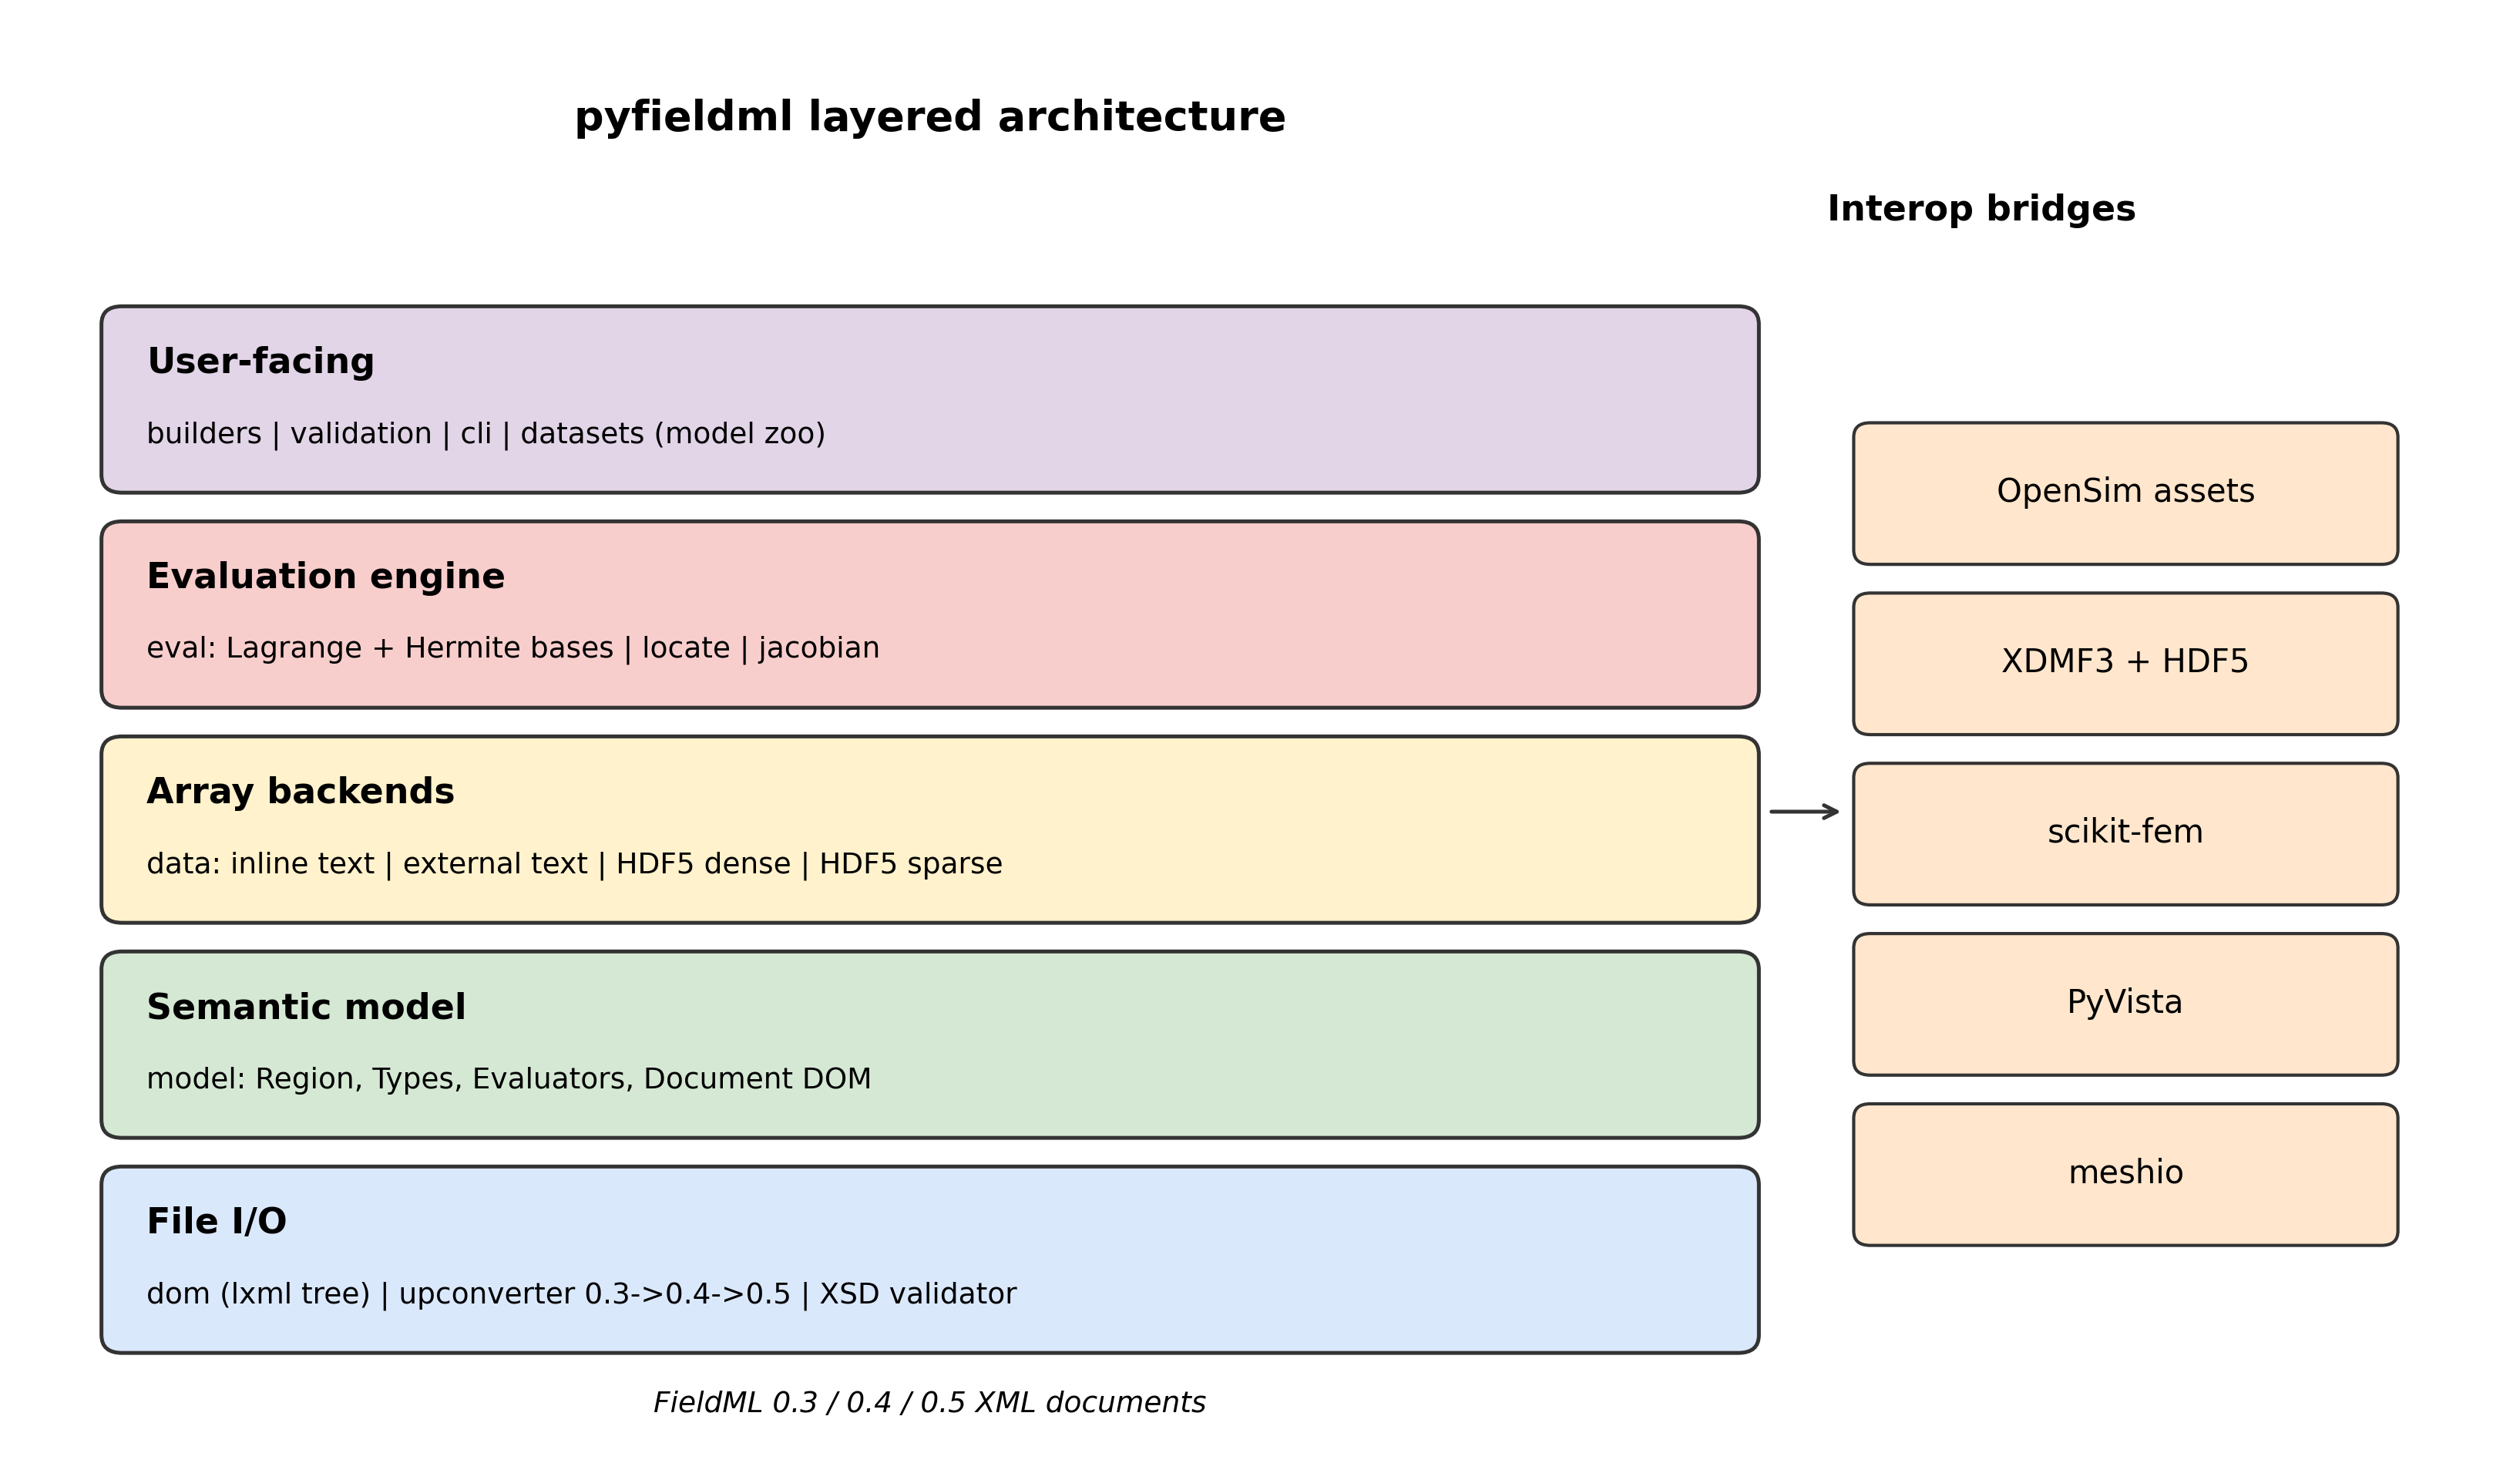
\includegraphics[width=0.98\textwidth]{figures/fig1_architecture.png}
\caption{Layered architecture of \texttt{pyfieldml}. The XML DOM layer handles FieldML 0.3/0.4/0.5 read/write and version up-conversion. The semantic model layer exposes a typed evaluator graph. The array-backend layer provides four independent storage paths (inline, external text, HDF5 dense, HDF5 sparse). The evaluation engine implements Lagrange and Hermite bases with spatial locate and Jacobian. The user-facing layer bundles builders, a validation linter, a CLI, and the ten-dataset model zoo. Interop bridges connect to the Python scientific stack.}
\label{fig:arch}
\end{figure}

Array data (parameter values, connectivity tables) is handled by the \texttt{data} layer, which provides four interchangeable backends---inline text, external text file, dense HDF5 \cite{hdf5,h5py}, and sparse HDF5 dictionary-of-keys---all exposed through a common \texttt{ndarray}-like interface with lazy loading and round-trip guarantees for \texttt{float32}, \texttt{float64}, \texttt{int32} and \texttt{int64}. The \texttt{eval} layer implements the evaluation engine: a plugin-based basis registry (12 Lagrange bases covering line/triangle/quadrilateral/tetrahedron/hexahedron/wedge at linear and quadratic order, and three cubic-Hermite bases on line/quad/hex with per-node scale factors), a spatial locate routine that inverts world $\rightarrow$ xi by Newton iteration, and a Jacobian calculator. \texttt{Field.evaluate(element, xi)}, \texttt{Field.sample(points)} and \texttt{Field.jacobian(element, xi)} are vectorised over NumPy \cite{numpy} arrays.

The user-facing layer contains \texttt{builders} (high-level constructors for common mesh/field patterns), a \texttt{validation} linter that flags orphan evaluators and inverted elements, a \texttt{cli} (\texttt{pyfieldml inspect\,|\,validate\,|\,convert\,|\,plot\,|\,lint\,|\,diff\,|\,bench}), and the \texttt{datasets} model zoo. Interop bridges are implemented as optional extras: \texttt{meshio} (two-way plugin), \texttt{PyVista} (\texttt{doc.plot()}), \texttt{scikit-fem} (returning a \texttt{(Mesh, Basis)} tuple ready for PDE assembly), \texttt{XDMF3}, and an OpenSim-adjacent asset exporter.

\subsection{Software functionalities}

The key functionalities of \texttt{pyfieldml} are: (i) read/write of FieldML 0.3/0.4/0.5 with transparent up-conversion, validated against the bundled XSD; (ii) an evaluator-graph DOM whose typed objects mirror the specification; (iii) an evaluation engine spanning 15 basis functions over six topologies with vectorised \texttt{evaluate}, \texttt{sample} and \texttt{jacobian}; (iv) a ten-dataset bundled model zoo (synthetic \texttt{unit\_cube}, \texttt{femur}, \texttt{rectus\_femoris}; Stanford Bunny \cite{stanford_bunny}; six real BodyParts3D \cite{bodyparts3d} skeletal segments: \texttt{femur\_bodyparts3d}, \texttt{tibia\_left}, \texttt{hip\_bone\_left}, \texttt{vertebra\_l3}, \texttt{scapula}, \texttt{skull}) shipped inside the wheel; (v) interop bridges to meshio, PyVista, XDMF3 and scikit-fem; (vi) a CLI and semantic linter; (vii) a SHA256-stamped reproducibility benchmark and a conformance workflow that cross-checks I/O against the C++ reference; (viii) an in-browser JupyterLite demo.

\subsection{Sample code snippet}

A complete load $\rightarrow$ evaluate $\rightarrow$ export round-trip fits in ten lines:

\begin{lstlisting}[style=pystyle]
import pyfieldml as fml

doc = fml.datasets.load("femur_bodyparts3d")   # BodyParts3D mesh
coords = doc.field("coordinates")              # evaluator graph
xyz = coords.evaluate(element=1, xi=(0.33, 0.33))
grid = doc.to_pyvista()                        # PyVista mesh
doc.to_meshio().write("femur.vtu")             # VTU export
fml.validation.lint(doc)                       # catch orphans
\end{lstlisting}

No FieldML-specific boilerplate is required; the document, its evaluator graph and its array data behave like first-class Python objects.

\section{Illustrative examples}

TODO: fill in three examples (model zoo, scikit-fem FEM, MSK assembly) in the next commit.

\section{Impact}

TODO: fill in next commit.

\section{Conclusions}

TODO: fill in next commit.

\section*{Acknowledgements}

The author thanks the Physiome Project community and the original FieldML authors (G.~Richard Christie, Caton Little, Alan Wu, Richard Christie, Andrew Miller, Poul Nielsen, Peter Hunter) for the conceptual foundation that \texttt{pyfieldml} builds on, and the Database Center for Life Science (DBCLS) Japan for maintaining BodyParts3D under a free license.

\bibliographystyle{elsarticle-num}
\bibliography{paper}

\end{document}
